\section{Atom--field interaction. Quantum approach}

\subsection{Jaynes–Cummings model (RWA)}

\begin{figure}[h!]
	\centering
	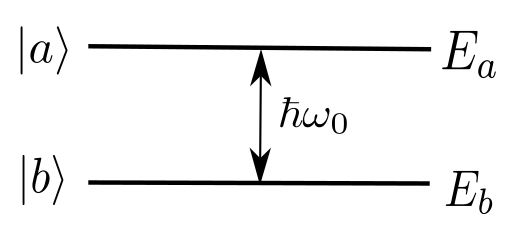
\includegraphics[width=0.3\linewidth]{fig/L6/2lvl}
	\caption{Two--level system}
	\label{fig:22lvl}
\end{figure}

Hamiltonian of system "quantum atom" $+$ "quantum field":
\begin{equation}
	\hat{\mathscr{H}} = \hat{\mathscr{H}}_A + \hat{\mathscr{H}}_F + \hat{\mathscr{H}}_{int}.
\end{equation}
where $\hat{\mathscr{H}}_A$ describes only \textit{atom}, $\hat{\mathscr{H}}_F$ describes only \textit{\textbf{quantised} field} and $\hat{\mathscr{H}}_{int}$ --- interaction part. Explicit expressions are:
\begin{eqnarray}
	\hat{\mathscr{H}}_A &=& E_a \ket{a} \bra{a} + E_b \ket{b} \bra{b}, \\
	\hat{\mathscr{H}}_F &=& \sum_{\vec{k}} \hbar \omega_{\vec{k}} \left( \hat{n}_{\vec{k}} + \frac{1}{2} \right), \qquad \hat{n}_{\vec{k}} = \hat{a}^{\dagger}_{\vec{k}} \hat{a}_{\vec{k}}, \\
	\hat{\mathscr{H}}_{\text{int}} &=& -e \vec{r} \cdot \hat{\vec{E}},
\end{eqnarray}
where field operator is given by
\begin{equation}
	\hat{\vec{E}} = \sum_{\kv} \varepsilon_{\kv} \left( \hat{a}_{\kv} \vec{e}_{\kv} e^{i \kv \vec{r}} + \hat{a}^{\dagger}_{\kv} \vec{e}^*_{\kv} e^{-i \kv \vec{r}} \right).
\end{equation}
For simplicity we consider case $\vec{k} = 0$ and $\vec{e}_{\kv} \in \mathbb{R}$ so we have
\begin{equation}
	\hat{\vec{E}} = \sum_{\vec{k}} \vec{e}_{\vec{k}} \varepsilon_{\kv} \left( \hat{a}^{\dagger}_{\kv} + \hat{a}_{\kv} \right).
\end{equation}
Now let us rewrite dipole moment:
\begin{equation}
	e \vec{r} = \hat{\mathbb{1}} \cdot e \vec{r} \cdot \hat{\mathbb{1}} = \sum_{i,j = a,b} \ket{i} \underbrace{\bra{i}  e \vec{r} \ket{j}}_{\vec{d}_{ij}} \bra{j} = \sum_{ij} \vec{d}_{ij} \underbrace{\ket{i} \bra{j}}_{\hat{\sigma}_{ij}} = \sum_{ij} \vec{d}_{ij} \hat{\sigma}_{ij}.
\end{equation}
Here we denoted:
\begin{equation}
	\vec{d}_{ij} \myeq \bra{i}  e \vec{r} \ket{j}, \qquad \hat{\sigma}_{ij} \myeq  \ket{i} \bra{j}.
\end{equation}
Then 
\begin{equation}
	\hat{\mathscr{H}}_{\text{int}} = - \sum_{ij} \sum_{\kv} \left(\vec{d}_{ij} \cdot \vec{e}_{\kv}\right) \sigma_{ij} \varepsilon_{\kv} \left( \hat{a}^{\dagger}_{\kv} + \hat{a}_{\kv} \right).
\end{equation}
Introduce a new notation:
\begin{equation}
	\boxed{	g_{ij}^{\kv} \myeq - \frac{ \varepsilon_{\kv} \left(\vec{d}_{ij} \cdot  \vec{e}_{\kv}\right)}{\hbar}.}
\end{equation}
This is a similarity to Rabi frequency but for one mode of field. To simplify computations let $g^{\kv}_{ij} \in \mathbb{R}$. So our Mr. Hamiltonian 
\begin{equation}
	\hat{\mathscr{H}} = E_a \hat{\sigma}_{aa} + E_b \hat{\sigma}_{bb} + \sum_{\vec{k}} \hbar \omega_{\kv} \left( \hat{a}^{\dagger}_{\kv} \hat{a}_{\kv} + \half \right) + \sum_{ij} \sum_{\kv} \hbar g_{ij}^{\kv} \hat{\sigma}_{ij} \left( \hat{a}^{\dagger}_{\kv} +  \hat{a}_{\kv} \right).
\end{equation}
\begin{figure}
	\centering
	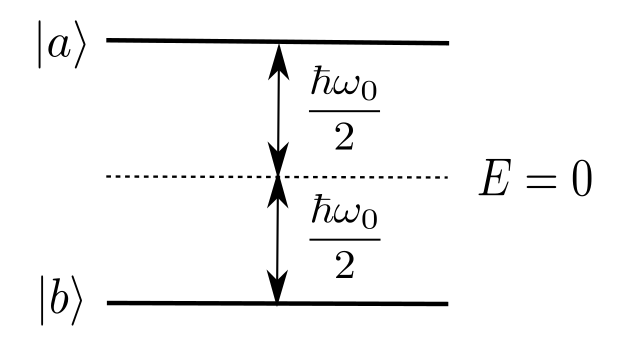
\includegraphics[width=0.4\linewidth]{fig/L6/E00000}
	\caption{A free choice of initial energy level}
	\label{fig:e00000}
\end{figure}
Let us put a starting energy point right in between $E_a$ and $E_b$ (fig.\ref{fig:e00000}). If we do so then
\begin{equation}
	E_a \hat{\sigma}_{aa} + E_b \hat{\sigma}_{bb} = \half \hbar \omega_0 \left( \hat{\sigma}_{aa} - \hat{\sigma}_{bb} \right) + \half \left( E_a + E_b \right)\underbrace{\left( \hat{\sigma}_{aa} + \hat{\sigma}_{bb} \right)}_{\hookrightarrow = \hat{\mathbb{1}}}.
\end{equation}
After that we make a transition to the new Hamiltonian by this energy shift
\begin{equation}
	\hat{\mathscr{H}} - \half \left( E_a + E_b \right) \quad \to \quad \hat{\mathscr{H}}.
\end{equation}

It is convenient to make new denotions:
\begin{eqnarray}
	\hat{\sigma}_{z} &\myeq& \hat{\sigma}_{bb} - \hat{\sigma}_{aa}, \\
	\hat{\sigma}_{+} &\myeq& \hat{\sigma}_{ab} = \ket{a} \bra{b}, \\
	\hat{\sigma}_{-} &\myeq& \hat{\sigma}_{ba} = \ket{b} \bra{a},
\end{eqnarray}
where
\begin{equation}
	\ket{b} = \begin{pmatrix}
		1 \\ 0
	\end{pmatrix}, \qquad
	\ket{a} = \begin{pmatrix}
	0 \\ 1
	\end{pmatrix},
\end{equation}
so reader may easily construct matrices for $\hat{\sigma}_{z}$, $\hat{\sigma}_{+}$ and $\hat{\sigma}_{-}$:
\begin{equation}
	\hat{\sigma}_z = \begin{pmatrix}
	1 & 0 \\ 0 & -1
	\end{pmatrix}, \qquad
	\hat{\sigma}_+ = \begin{pmatrix}
	0 & 0 \\ 1 & 0
	\end{pmatrix}, \qquad
	\hat{\sigma}_- = \begin{pmatrix}
	0 & 1 \\ 0 & 0
	\end{pmatrix}.
\end{equation}
To answer how act new operators $\hat{\sigma}_{+}$ and $\hat{\sigma}_{-}$ consider the following:
\begin{eqnarray}
	\hat{\sigma}_{+} \ket{b} = \ket{a} \braket{b}{b} = \ket{a}, \\
	\hat{\sigma}_{-} \ket{a} = \ket{b} \braket{a}{a} = \ket{b}.
\end{eqnarray}
The operator $\hat{\sigma}_{+}$ takes the system lower state to upper states vice versa.

Usually $\vec{d}_{aa} = \vec{d}_{bb} = 0$, so
\begin{equation}
	g^{\kv}_{aa} = 0, \qquad g^{\kv}_{bb} = 0,
\end{equation}
\begin{equation}
	g^{\kv}_{ab} = g^{\kv}_{ba} \myeq g^{\kv}.
\end{equation}
After that Hamiltonian may be written as 
\begin{equation}
	\hat{\mathscr{H}} = \underbrace{\sum_{\kv} \hbar \omega_{\kv} \left( \hat{a}_{\kv}^{\dagger}\hat{a}_{\kv} + \half \right)}_{\text{field}} + \underbrace{\frac{\hbar \omega_0}{2} \hat{\sigma}_z}_{\text{atom}} + \underbrace{\hbar \sum_{\kv} g^{\kv} \left( \hat{\sigma}_+ + \hat{\sigma}_- \right) \left( \hat{a}^{\dagger}_{\kv} + \hat{a}_{\kv} \right)}_{\text{interaction}}.
\end{equation}

Algebra of new operators:
\begin{eqnarray}
	\left[ \hat{\sigma}_-, \hat{\sigma}_+ \right] &=& - \hat{\sigma}_z, \\
	\left[ \hat{\sigma}_-, \hat{\sigma}_z \right] &=& 2\hat{\sigma}_-, \\
	\left[ \hat{\sigma}_+, \hat{\sigma}_z \right] &=& -2 \hat{\sigma}_+, \\
	\left\{ \hat{\sigma}_+, \hat{\sigma}_- \right\} &=& \hat{\mathbb{1}}.
\end{eqnarray}
Last property is rooted in fact that electrons are fermions. $\hat{\sigma}_+$ and $\hat{\sigma}_-$ are creation and annihilation operators for electron in atom. Lets consider the physical meaning of the interactive terms:
\begin{equation}
	\left( \hat{\sigma}_+ + \hat{\sigma}_- \right) \left( \hat{a}^{\dagger}_{\kv} + \hat{a}_{\kv} \right) = \underbrace{\hat{\sigma}_+ \hat{a}}_{\text{(I)}} + \overbrace{\underbrace{\cancel{\hat{\sigma}_+ \hat{a}^{\dagger}}}_{\text{(II)}} + \underbrace{\cancel{\hat{\sigma}_- \hat{a}}}_{\text{(III)}}}^{\text{unphysical}} + \underbrace{\hat{\sigma}_- \hat{a}^{\dagger}}_{\text{(IV)}},
\end{equation}
where (I) --- photon annihilation and electron excitation, (II) --- photon creation and electron excitation, (III) --- photon annihilation and electron relaxation, (IV) --- photon creation and electron relaxation. Terms  $\hat{\sigma}_+\hat{a}^{\dagger} + \hat{\sigma}_-\hat{a}$ are unphysical, so \textit{may be omitted}. In fact this is the RWA. After such assumption we have:
\begin{equation}
	\boxed{\hat{\mathscr{H}} = \sum_{\kv} \hbar \omega_{\kv} \left( \hat{a}_{\kv}^{\dagger}\hat{a}_{\kv} + \half \right) + \frac{\hbar \omega_0}{2} \hat{\sigma}_z + \sum_{\kv} \hbar g^{\kv} \left( \hat{\sigma}_+\hat{a}_{\kv} + \hat{a}^{\dagger}_{\kv} \hat{\sigma}_- \right).}
\end{equation}

For simplicity let us consider one mode field
\begin{equation}
	\hat{\mathscr{H}} = \underbrace{\hbar \omega \left( \hat{a}^{\dagger}\hat{a} + \half \right) + \frac{\hbar \omega_0}{2} \hat{\sigma}_z}_{\hat{\mathscr{H}}_0} + \underbrace{\hbar g \left( \hat{\sigma}_+\hat{a} + \hat{a}^{\dagger} \hat{\sigma}_- \right)}_{\hat{V}}.
	\label{eq:hamillll}
\end{equation}
Now we go in the interaction representation
\begin{equation}
	\hat{\mathscr{H}}_V = e^{\frac{i}{\hbar} \hat{\mathscr{H}}_0 t} \hat{V} e^{-\frac{i}{\hbar} \hat{\mathscr{H}}_0 t}.
\end{equation}
\begin{enumerate}
	\item[\textit{Remark}:] \textit{The interaction representation means the following. 
	After unitary transformation }
	\begin{equation*}
	\ket{\widetilde{\psi}} = e^{\frac{i}{\hbar} \hat{\mathscr{H}}_0 t} \ket{\psi}, \qquad \hat{\mathscr{H}} \to \hat{\mathscr{H}}_V
	\end{equation*}
	\textit{we obtain new effective Schrödinger equation}
	\begin{equation*}
	i \hbar \dot{\ket{\psi}} = \hat{\mathscr{H}} \ket{\psi} \quad \to \quad i \hbar \dot{\ket{\widetilde{\psi}}} = \hat{\mathscr{H}}_V \ket{\widetilde{\psi}}.
	\end{equation*}   
\end{enumerate}
Let us begin. We need to consider
\begin{equation}
	e^{i \frac{\omega_0}{2} \hat{\sigma}_z t} e^{i \omega \hat{a}^{\dagger} \hat{a} t} \hat{V} e^{-i \omega \hat{a}^{\dagger} \hat{a} t} e^{-i \frac{\omega_0}{2} \hat{\sigma}_z t}.
\end{equation}
Different terms will appear:
\begin{eqnarray}
	e^{i \omega \hat{a}^{\dagger} \hat{a} t} \hat{a} e^{-i \omega \hat{a}^{\dagger} \hat{a} t} &=& \hat{a} e^{- \omega t}, \\
	e^{i \omega \hat{a}^{\dagger} \hat{a} t} \hat{a}^{\dagger} e^{-i \omega \hat{a}^{\dagger} \hat{a} t} &=& \hat{a}^{\dagger} e^{i \omega t}, \\
	e^{i \frac{\omega_0}{2} \hat{\sigma}_z t} \hat{\sigma}_+ e^{-i \frac{\omega_0}{2} \hat{\sigma}_z t} &=& \hat{\sigma}_+ e^{i \omega_0 t}, \\
	e^{i \frac{\omega_0}{2} \hat{\sigma}_z t} \hat{\sigma}_- e^{-i \frac{\omega_0}{2} \hat{\sigma}_z t} &=& \hat{\sigma}_- e^{-i \omega_0 t}.
\end{eqnarray}
So
\begin{equation}
	\hat{\mathscr{H}}_V = \hbar g \left( \hat{a}^{\dagger} \hat{\sigma}_- e^{-i (\omega_0 - \omega)t} + \hat{\sigma}_+ \hat{a} e^{i (\omega_0 - \omega)t} \right).
\end{equation}
As a matter of convenience we introduce $\Delta \myeq \omega_0 - \omega$. An effective Schrödinger equation now may be written as
\begin{equation}
	\quad i \hbar \parder{}{t}\ket{\widetilde{\psi}} = \hat{\mathscr{H}}_V \ket{\widetilde{\psi}}.
\end{equation}
After that we expand wave function in series 
\begin{equation}
	\ket{\widetilde{\psi}} = \sum_{n} C_{a,n}(t) \ket{n} \ket{a} + \sum_{n} C_{b,n}(t) \ket{n} \ket{b},
\end{equation}
where $C_{a,n}(t)$ --- a probability of finding an electron in $\ket{a}$ and a photon in $\ket{n}$ at time $t$. To bring into focus results we omit all the computations and present only the solution:
\begin{equation}
	\begin{cases}
		i \hbar \dot{C}_{a,n}(t) = \hbar g \sqrt{n+1} C_{b,n+1}(t) e^{i \Delta t}, \\
		i \hbar \dot{C}_{b,n+1}(t) = \hbar g \sqrt{n+1} C_{a,n}(t) e^{-i \Delta t}.
	\end{cases}
	\label{eq:228_botat_my_ne_brosim}
\end{equation}

\begin{figure}
	\centering
	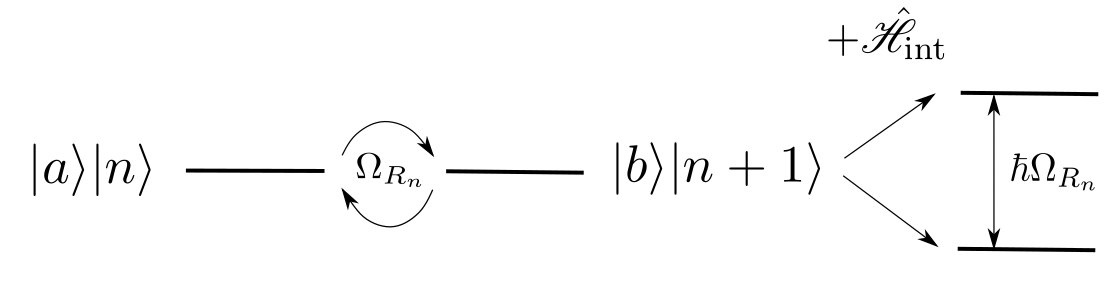
\includegraphics[width=0.8\linewidth]{fig/L6/E_split}
	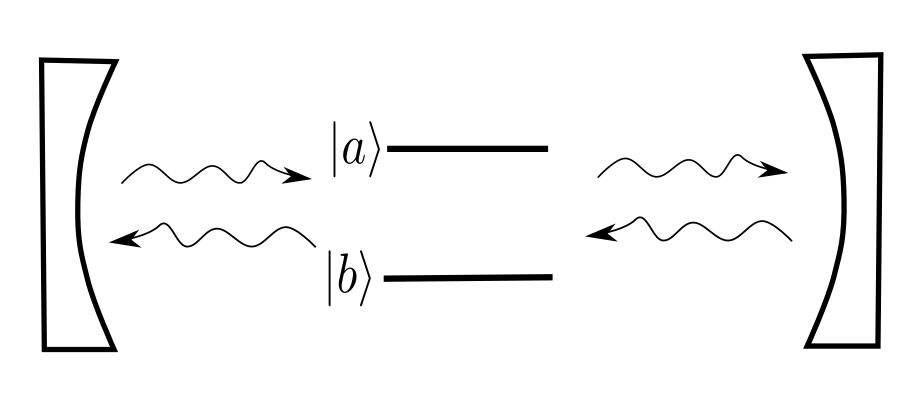
\includegraphics[width=0.5\linewidth]{fig/L6/osc_in_cavity}
	\caption{Oscillations in a cavity}
	\label{fig:228}
\end{figure}


For simplicity let us consider a resonant excitation, it means we need to put $\Delta  =0$ in \eqref{eq:228_botat_my_ne_brosim}. After we have
\begin{equation}
	\begin{cases}
		\dot{C}_{a,n}(t) = -i g \sqrt{n+1} C_{b,n+1}(t) \\
		\dot{C}_{b,n+1}(t) = -i g \sqrt{n+1} C_{a,n}(t)
	\end{cases} \qquad \to \qquad 
	\ddot{C}_{a,n} (t) + \underbrace{g^2(n+1)}_{\Omega_{R_n}^2} C_{a,n}(t) = 0.
\end{equation}
Easy to notice, we obtained osculations with angular frequency 
\begin{equation}
	\boxed{\Omega_{R_n} = g \sqrt{n+1}.}
\end{equation}
A physical interpretation of such oscillations is shown in fig. \ref{fig:228}.

\begin{testexample}[Vacuum Rabi oscillations.]
	If we put $n=0$ we get $\Omega_{R_0} = g \neq 0$. We have a vacuum interaction: no field, interaction exists!
	%\textcolor{red}{(UNCOMMENT THIS LATER! (see source))}
\end{testexample}

\subsection{Collapse and revival}

Another important quantity is the inversion $W(t)$ which is related to the probabilty amplitudes $C_{a,n}(t)$ and $C_{b,n}(t)$ by the expression
\begin{equation}
	W(t) = \sum_{n} \left( \left| C_{a,n}(t) \right|^2 - \left| C_{b,n}(t) \right|^2 \right).
\end{equation}
In fig. \ref{fig:candr} $W(t)$ is plotted as a function of normalized time $g t$ for an initial coherent state. The behavior of $W(t)$ is quite different from the corresponding curve (fig. \ref{fig:rabiosc}) in the semiclassical theory. In the present case the envelope of the sinusoidal Rabi oscillations '\textit{collapses}' to zero. However as time increases we encounter a '\textit{revival}' of the collapsed inversion. This behavior of collapse and revival of inversion is repeated with increasing time, with the amplitude of Rabi osculations decreasing and the time duration in which revival takes place increasing and ultimately overlapping with the earlier revival.

\begin{figure}
	\centering
	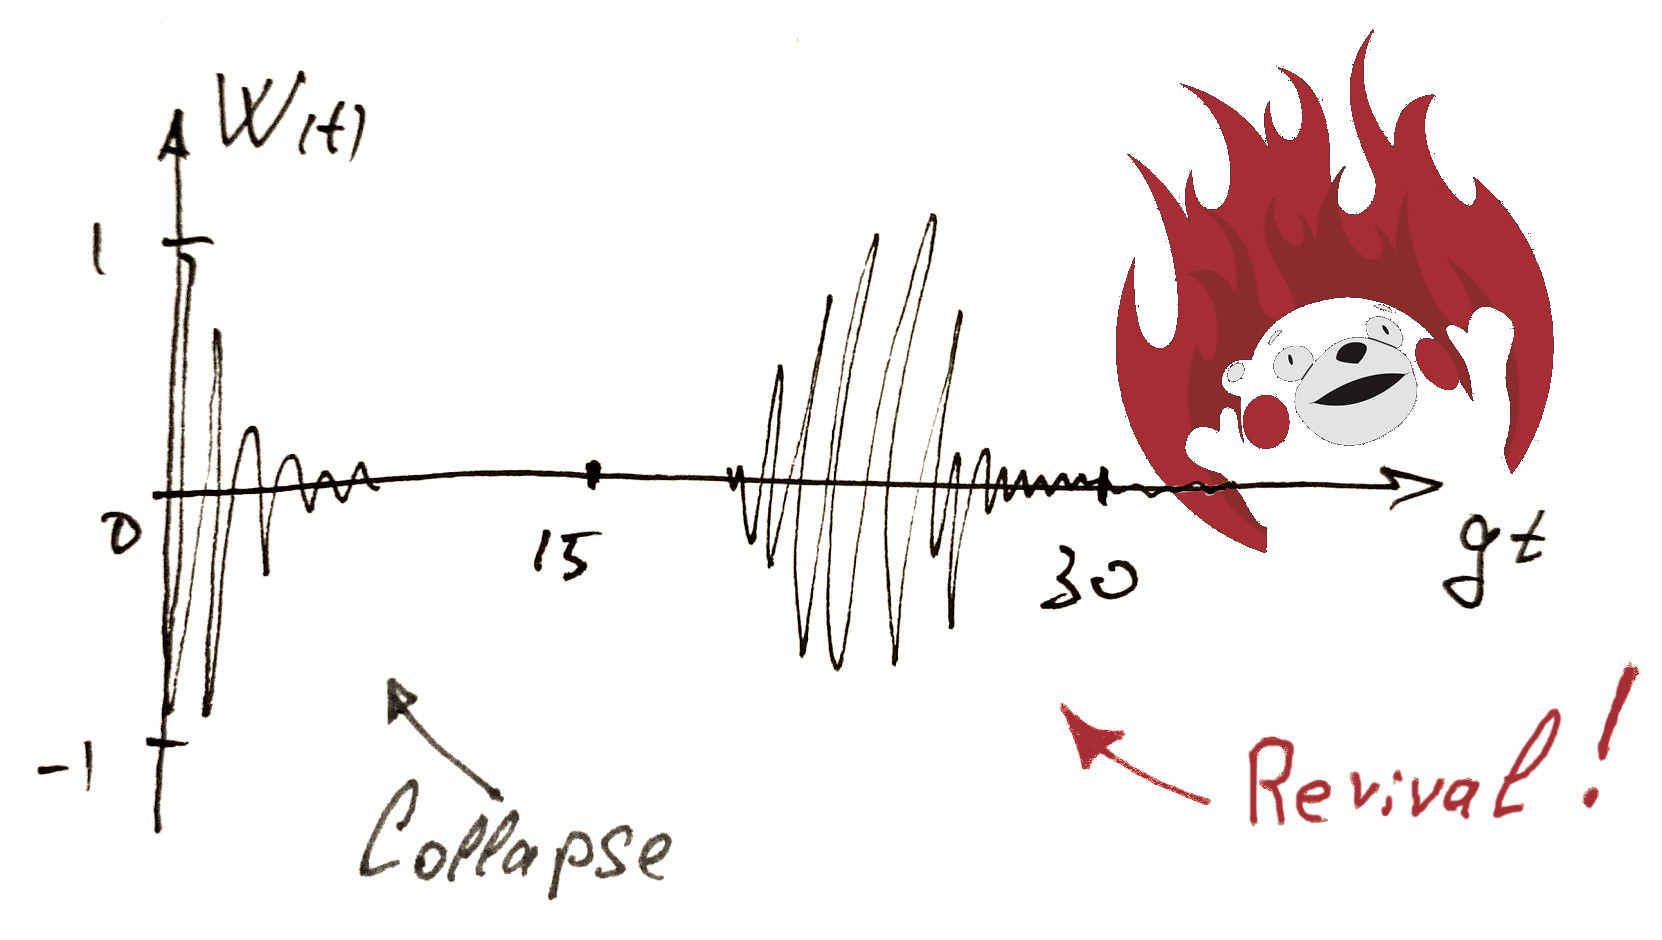
\includegraphics[width=0.7\linewidth]{fig/L6/c_and_r.jpg}
	\caption{Time evolution of the population inversion $W(t)$ for an initially coherent state.}
	\label{fig:candr}
\end{figure}


\subsection{Energy spectrum. Dispersion relation}

Let us find eigenstates of $\hat{\mathscr{H}}$ which is given by \eqref{eq:hamillll}. Here, for convenience, the vacuum field energy is set to $0$, so
\begin{equation}
	\hat{\mathscr{H}} = \underbrace{\hbar \omega  \hat{n} + \frac{\hbar \omega_0}{2} \hat{\sigma}_z}_{\hat{\mathscr{H}}_0} + \underbrace{\hbar g \left( \hat{\sigma}_+\hat{a} + \hat{a}^{\dagger} \hat{\sigma}_- \right)}_{\hat{\mathscr{H}}_{\text{int}}}.
\end{equation}

The equation for eigenvalues is 
\begin{equation}
\hat{\mathscr{H}} \ket{\psi} = E \ket{\psi}.
\label{eq:eigen} 
\end{equation}
Next terms will appear:
\begin{eqnarray}
	\hat{\mathscr{H}}_0 \ket{a} \ket{n} &=& \left( \frac{\hbar \omega_0}{2} + \hbar \omega n \right) \ket{a} \ket{n}, \\
	\hat{\mathscr{H}}_0 \ket{b} \ket{n+1} &=& \left( -\frac{\hbar \omega_0}{2} + \hbar \omega n \right) \ket{b} \ket{n+1}, \\
	\hat{\mathscr{H}}_{\text{int}} \ket{a} \ket{n} &=& \hbar g \sqrt{n+1} \ket{b} \ket{n+1}, \\
	\hat{\mathscr{H}}_{\text{int}} \ket{b} \ket{n+1} &=& \hbar g \sqrt{n+1} \ket{a} \ket{n}.
\end{eqnarray}
Important to notice that number of quantas is concerned, if we take  basis $\ket{a} \ket{n}$ and $\ket{b} \ket{n+1}$. After acting $\hat{\mathscr{H}}_{\text{int}}$ we stay in the same subspace with the same basis. Consequently, eigenfunctions may be written as
\begin{equation}
	\ket{\psi} = \ket{\varphi_1} \cdot \ket{\varphi_2} \cdot ... \cdot \ket{\varphi_n} \cdot ...
\end{equation}
Each of $\ket{\varphi_n}$ acts on its own subspace and does not affect the others:
\begin{equation}
	\ket{\varphi_n} = c_n \ket{a} \ket{n} + c_{2n} \ket{b} \ket{n+1}.
\end{equation}
It leads to a very imports consequence --- $\hat{\mathscr{H}}$ is \textit{block-diagonal matrix}:
\begin{equation}
	\hat{\mathscr{H}} = 
	\begin{pmatrix}
		\hat{\mathcal{H}}_1 & 0 & 0 & \dots & 0 & \dots \\
		0& \hat{\mathcal{H}}_2 &0 & \dots &0 & \dots\\
		\vdots & \dots  & \ddots & \dots & \vdots & \dots \\
		0 & \dots & 0& \hat{\mathcal{H}}_n & 0 & \dots \\
		\vdots & \vdots & \vdots & \ddots & \ddots & \ddots
	\end{pmatrix}.
\end{equation}
Where each of $\hat{\mathcal{H}}_n$ is a $2\times2$ matrix.

Looking for an energy spectrum \eqref{eq:eigen} is equivalent to the Hamiltonian diagonalization.
We simplified our problem and now we need only to diagonalize $2 \times 2$ matrices or in other words we need to solve
\begin{equation}
	\hat{\mathcal{H}}_n \ket{\varphi_n} = E_n \ket{\varphi_n}.
\end{equation}

In an explicit form we need to diagonalize
\begin{multline}
	\hat{\mathcal{H}}_n = \hat{\mathcal{H}}^0_{n} + \hat{\mathcal{H}}^{\text{int}}_n = 
	\begin{pmatrix}
		\frac{\hbar \omega_0}{2} + \hbar \omega n & 0 \\
		0 & - \frac{\hbar \omega_0}{2} + \hbar \omega n
	\end{pmatrix} +
	\begin{pmatrix}
		0 & \hbar g \sqrt{n+1} \\
		\hbar g \sqrt{n+1} & 0
	\end{pmatrix} = \\ \\ =
	\hbar \omega \left( n+ \half \right) \hat{I}
	+ \frac{\hbar}{2} \begin{pmatrix}
		\Delta & 2g \sqrt{n+1} \\ \\
		2g \sqrt{n+1} & - \Delta
	\end{pmatrix},
\end{multline}
where $\Delta = \omega - \omega_0$ and $\hat{I} = \begin{pmatrix}
1 & 0 \\
0 & 1
\end{pmatrix}$ is an identity matrix. Human by nature is lazy, so we do. It means let us consider a simple case when $\Delta = 0$, so
\begin{equation}
	\det \left( \hat{\mathcal{H}}_n - E \hat{I} \right) = 0 \quad \to \quad \left( E - \hbar \omega (n + \half) \right) = \hbar^2 g^2 (n+1)
\end{equation} 
or
\begin{equation}
	\begin{cases}
		E_1 = \hbar \omega \left( n + \half \right) + \hbar g \sqrt{n+1}, \\
		E_2 = \hbar \omega \left( n + \half \right) - \hbar g \sqrt{n+1}.
	\end{cases}
\end{equation}
\begin{figure}
	\centering
	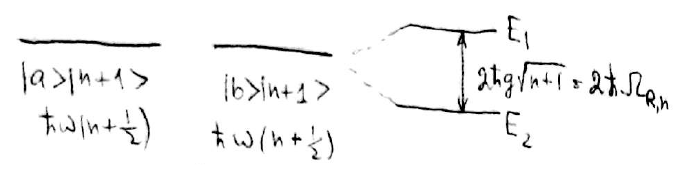
\includegraphics[width=0.7\linewidth]{fig/L6/leveeeelllls}
	\caption{Level splitting after acting $\hat{\mathcal{H}}_n$}
	\label{fig:leveeeelllls}
\end{figure}
This energy splitting is shown in fig. \ref{fig:leveeeelllls}. If we consider case $\Delta \neq 0$ then we will get
\begin{equation}
	\begin{cases}
	E_1 = \hbar \omega \left( n + \half \right) + \half \hbar R_n, \\
	E_2 = \hbar \omega \left( n + \half \right) - \half \hbar R_n,
	\end{cases}
	\label{eq:system57}
\end{equation}
where $R_n = \sqrt{\Delta^2 + 4g^2 (n+1)}$.
\begin{figure}
	\centering
	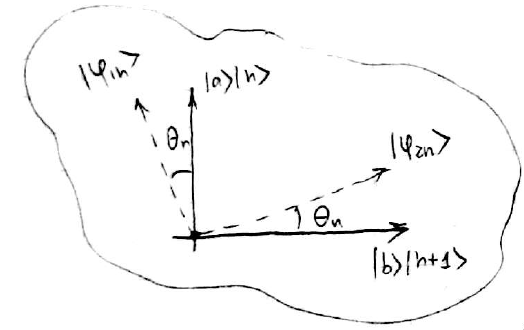
\includegraphics[width=0.65\linewidth]{fig/L6/rotation}
	\caption{Rotation in a subspace}
	\label{fig:rotation}
\end{figure}

Eigenstates may be written as a rotated $\ket{a,n}$ and $\ket{b,n+1}$ states
\begin{equation}
	\begin{cases}
		\ket{\varphi_{1n}} = \cos \vartheta_n \ket{a, n} + \sin \vartheta_n \ket{b ,n +1}, \\
		\ket{\varphi_{2n}} = -\sin \vartheta_n \ket{a, n} + \cos \vartheta_n \ket{b ,n +1},
	\end{cases}
\end{equation}
where $\cos \vartheta_n = \frac{2 g \sqrt{n+1}}{\sqrt{(R_n - \Delta)^2 + 4 g^2 (n+1)}}$. Just to make things clear, $\ket{a,n}$ and $\ket{b,n+1}$ are eigenfunctions of $\hat{\mathcal{H}}^0_{n}$, after 'turning on' an interaction we gain a plane rotation!


States $\ket{\varphi_{1n}}$ and $\ket{\varphi_{2n}}$ --- \textit{polariton states}. This is a mixed stated of light and medium. 


For $\Delta = 0$ we have $\vartheta = \frac{\pi}{4}$. It means that
\begin{equation}
	\begin{cases}
		\ket{\varphi_{1n}} = \frac{1}{\sqrt{2}} \left(\ket{a, n} + \ket{b ,n +1}\right), \\
		\ket{\varphi_{2n}} = \frac{1}{\sqrt{2}}\left(-\ket{a, n} + \ket{b ,n +1}\right).
	\end{cases}
\end{equation}
Energy is given by \eqref{eq:system57}. If there is no interaction ($g = 0$) we have
\begin{equation}
	\begin{cases}
		E_{1n} = \hbar \omega \left( n + \half\right) + \frac{\hbar}{2} \Delta, \\
		E_{2n} = \hbar \omega \left( n + \half\right) - \frac{\hbar}{2} \Delta.
	\end{cases}
\end{equation}
Not let us make a graphical analysis. At first shall we put $n=0$ and $g=0$ (fig. \ref{fig:n0}). After that we 'turn on' interaction ($n=0$, $g \neq 0$) and we get fig. \ref{fig:n0gne0}. All necessary comments are given under the figures.

\begin{figure}
	\centering
	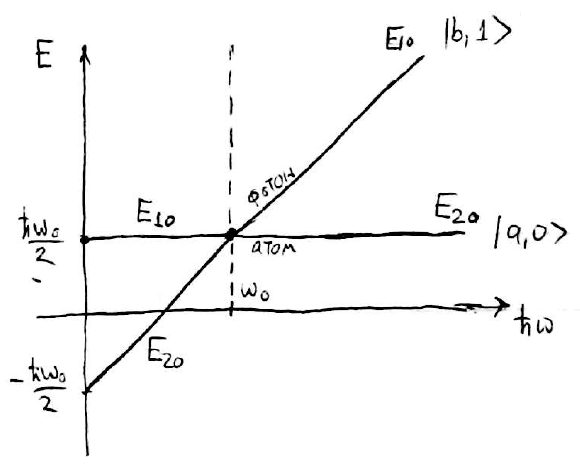
\includegraphics[width=0.5\linewidth]{fig/L6/n0}
	\caption{Case of $n=0$ and $g=0$. State $\ket{b,1}$ --- there is a photon with energy $\hbar \omega$, so $E = E(\omega)$ is linear. State $\ket{a,0}$ --- no photon in cavity, energy does not depend on $\hbar \omega$, there is an exciton}
	\label{fig:n0}
\end{figure}
\begin{figure}
	\centering
	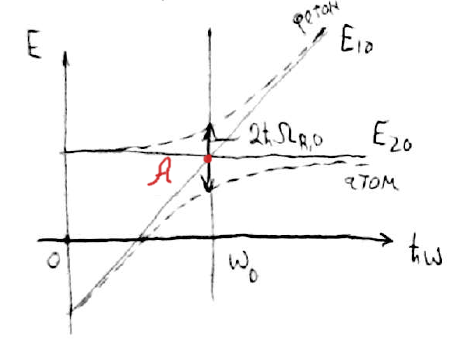
\includegraphics[width=0.5\linewidth]{fig/L6/n0_g_ne0}
	\caption{Case of $n=0$ and $g\neq0$. Line splitting is observed. At frequency $\omega_0$ there is no pure atom state nor photon state --- it is mixed state, polariton state}
	\label{fig:n0gne0}
\end{figure}

At point A on fig. \ref{fig:n0gne0} quantum of energy neither in atom nor in photon, it is equidistant from $E_{01}$ and $E_{02}$. This is a \textit{polariton state}!

In fact we described a so called Cummings ladder (fig. \ref{fig:lad}).
\begin{figure}
	\centering
	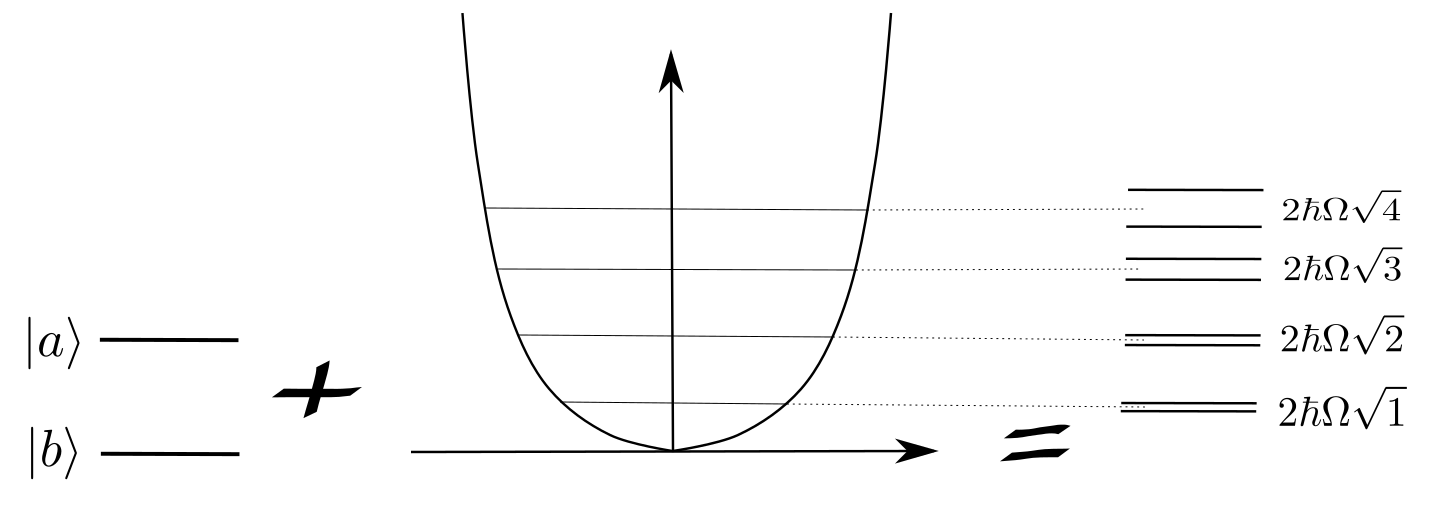
\includegraphics[width=0.6\linewidth]{fig/L6/lad}
	\caption{Cummings ladder. Energy splitting as a result of combining two quantum systems: atom and field}
	\label{fig:lad}
\end{figure}
